% ============================================================
%  CHAPITRE 4 — Section 6 : Synthèse comparative
% ============================================================

\section{Synthèse comparative}
\label{sec:synthese_ch4}

Les trois axes d'augmentation ont été développés séparément, puis combinés. Cette section les replace dans une vue d'ensemble, situe les stratégies augmentées les unes par rapport aux autres et vis-à-vis du front optimal, et dégage l'apport propre à chaque connaissance.

% ------------------------------------------------------------
\subsection{Vue d'ensemble dans le plan de Pareto}
% ------------------------------------------------------------

Le Tableau~\ref{tab:synthese} rassemble les performances des stratégies de ce chapitre, et la Figure~\ref{fig:pareto_synthese} les positionne dans le plan de Pareto, avec le front optimal par programmation dynamique introduit au chapitre précédent comme repère.

\begin{table}[h!]
\centering
\caption{Synthèse des stratégies augmentées. Les stratégies prévisionnelles sont des moyennes Monte-Carlo sous bruit de prévision réaliste. Le front optimal est la borne par programmation dynamique du chapitre précédent.}
\label{tab:synthese}
\begin{tabular}{llccc}
\hline
Stratégie & Connaissance mobilisée & LPSP [\%] & Dégradation [k€] & Coût total [k€] \\
\hline
RB2 (référence)   & --- (réactive)                       & 2,59 & 58,85 & 80,11 \\
RB2(RUL)          & durée de vie résiduelle              & 2,59 & 58,85 & 80,11 \\
RB2(Pred)         & prévision de profils                 & 2,53 & 58,96 & 79,72 \\
\RBsohB           & SoH de la batterie                   & 2,77 & 56,84 & 79,54 \\
\RBsohH           & SoH de la pile et de l'électrolyseur & 2,91 & 54,91 & 78,77 \\
\RBsohA           & état de santé des trois stockeurs    & 3,11 & 52,87 & 78,34 \\
\RBshp            & santé hydrogène et prévision         & 2,76 & 55,08 & 77,69 \\
\RBult            & santé complète et prévision          & \textbf{2,94} & \textbf{53,10} & \textbf{77,22} \\
\hline
\end{tabular}
\end{table}

\begin{figure}[h!]
    \centering
    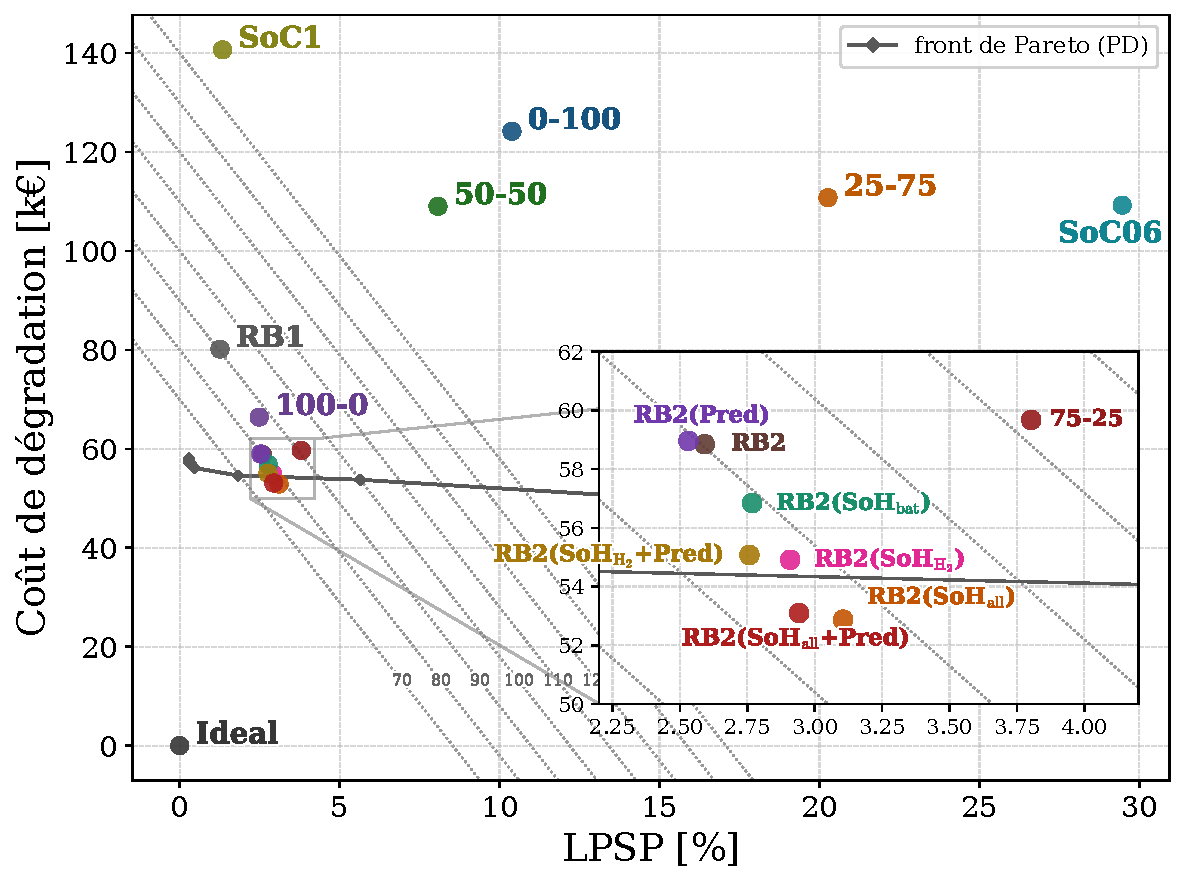
\includegraphics[width=\linewidth]{Chapitre 3/Synthese/Figures/pareto_strategies_v2.pdf}
    \caption{Positionnement des stratégies augmentées dans le plan de Pareto LPSP--coût de dégradation, vis-à-vis de la référence RB2 et du front de Pareto optimal par programmation dynamique~; agrandissement sur la famille RB2 en encart. Les stratégies s'échelonnent le long d'une direction isocoût, de RB2(Pred) (la plus fiable) à \RBsohA{} (la plus durable), la stratégie complète \RBult{} réalisant le meilleur coût total.}
    \label{fig:pareto_synthese}
\end{figure}
\FloatBarrier

L'incertitude des stratégies prévisionnelles est faible à l'échelle du plan d'ensemble. Elle est représentée séparément sur un zoom dédié à chaque paire, sous forme d'ellipses d'incertitude $1\sigma/2\sigma$ autour de la moyenne Monte-Carlo (Figure~\ref{fig:pareto_zoom})~: dans les trois cas, la dispersion induite par le bruit de prévision est petite devant l'écart avec la base sans prévision --- les ellipses à $2\sigma$ n'atteignent jamais la base --- si bien que le gain est acquis quelle que soit la réalisation du bruit.

\begin{figure}[h!]
    \centering
    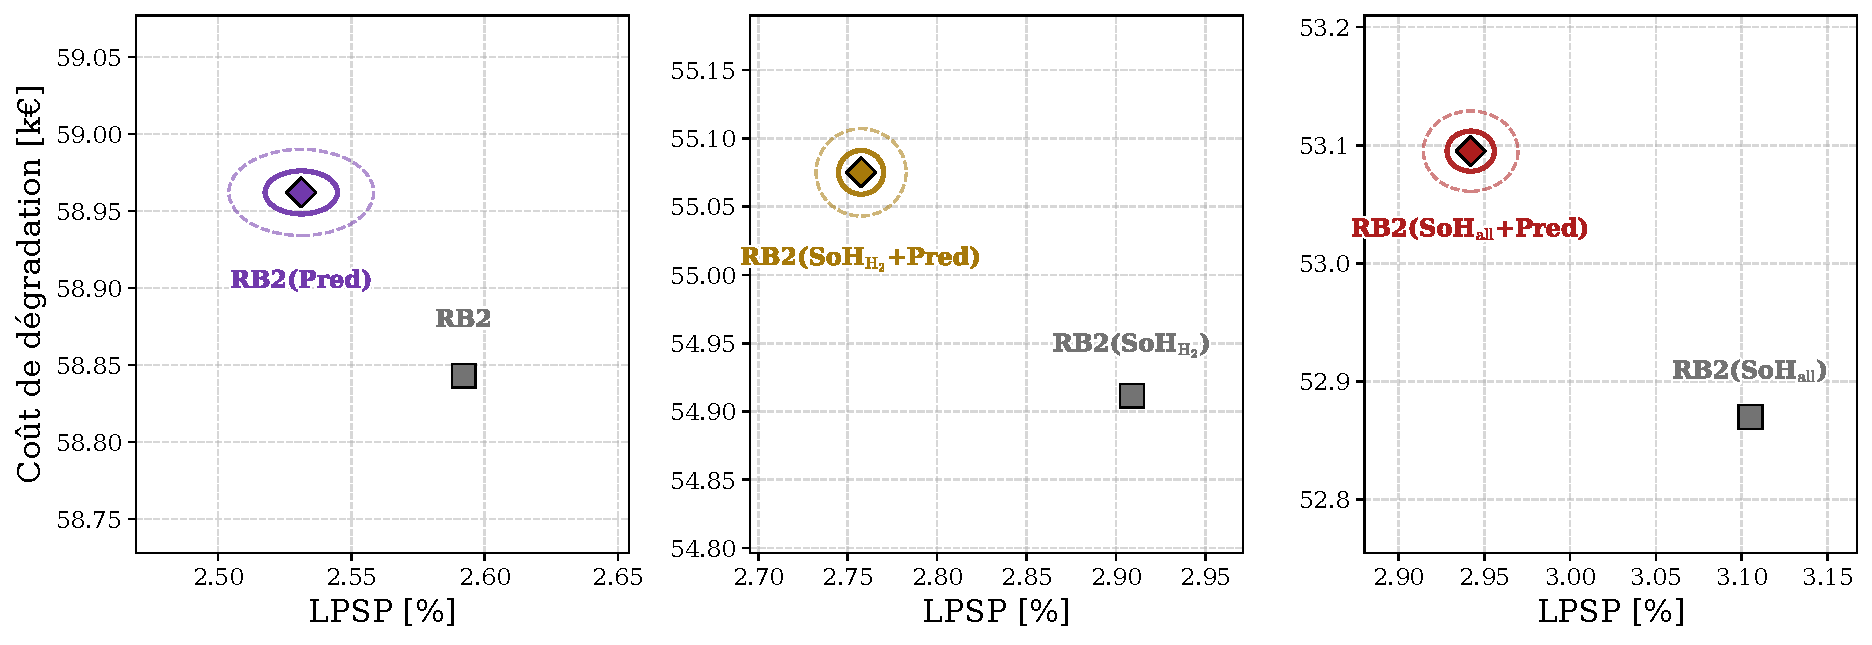
\includegraphics[width=\linewidth]{Chapitre 3/Synthese/Figures/pred_uncertainty_zoom_v2.pdf}
    \caption{Zoom sur les trois stratégies prévisionnelles et leur incertitude Monte-Carlo ($N=200$, ellipses $1\sigma$ en trait plein, $2\sigma$ en tirets), chacune face à sa base sans prévision (carré gris).}
    \label{fig:pareto_zoom}
\end{figure}
\FloatBarrier

% ------------------------------------------------------------
\subsection{Apport de chaque connaissance}
% ------------------------------------------------------------

La vue d'ensemble fait apparaître une répartition des rôles entre les connaissances, cohérente avec la grandeur sur laquelle chacune agit.

\begin{itemize}
  \setlength\itemsep{2pt}
  \item L'état de santé agit sur la durabilité, par deux leviers indépendants et additifs. Le levier hydrogène (\RBsohH) abaisse le coût de dégradation d'environ $6{,}7\,\%$ (de $58{,}85$ à $54{,}91$~k€) en ménageant l'électrolyseur vieillissant, pour un gain de $1{,}34$~k€ sur le coût total. Le levier batterie (\RBsohB) referme progressivement la fenêtre de SoC avec l'usure et apporte $0{,}56$~k€, avec un bassin d'optimum plat qui en fait un réglage robuste. Leur cumul (\RBsohA) restitue $93\,\%$ de la somme des gains individuels ($-1{,}77$~k€ au total), signe que les deux leviers exploitent des gisements physiquement distincts~; \RBsohA{} constitue la meilleure stratégie sans prévision du chapitre ($78{,}34$~k€).
  \item La prévision agit sur la fiabilité~: RB2(Pred) améliore la LPSP à dégradation quasi constante, en anticipant les creux de production par la pré-charge de la batterie ($80{,}11 \to 79{,}72$~k€). Son apport croît avec la qualité du socle sur lequel elle se greffe~: $0{,}38$~k€ sur RB2, mais $1{,}08$~k€ sur \RBsohH{} et $1{,}11$~k€ sur \RBsohA, car la pré-charge évite des démarrages d'électrolyseur dont le coût unitaire pèse davantage dans un système déjà optimisé pour la durabilité.
  \item Le pronostic n'apporte, lui, aucun gain~: une fois le socle de RB2 optimisé, le balayage des paramètres de RB2(RUL) retient un exposant nul, si bien que RB2(RUL) se confond exactement avec RB2. La durée de vie résiduelle, redondante avec le SoH et peu fiable en début de vie, n'ajoute pas d'information exploitable au-delà du diagnostic.
  \item La stratégie complète \RBult{} cumule l'ensemble des leviers validés et réalise le meilleur coût total du chapitre ($77{,}22$~k€, soit $-3{,}7\,\%$ par rapport à RB2), sous réserve d'asservir les seuils de la règle prévisionnelle à la fenêtre de SoC vieillissante --- faute de quoi l'interaction entre les deux leviers détruit le gain du levier batterie.
\end{itemize}

Ces apports sont modestes en valeur absolue mais attribuables~: la propriété de test nul, appliquée à socle optimisé (comparaison « best-vs-best »), garantit que chaque écart provient de la connaissance ajoutée, et non d'un socle mal réglé ni d'une refonte de la logique de contrôle. Ils dessinent en creux une hiérarchie de l'information~: l'état présent (SoH) vaut davantage que le futur de l'environnement (prévision), qui vaut davantage que le futur extrapolé du composant (RUL), nul une fois le diagnostic exploité. Il est également notable que chaque gain de durabilité se paie d'une concession mesurée de fiabilité~: aucun levier ne dégage de marge « gratuite », ce qui confirme que le socle RB2 opère déjà près de son propre front. Vis-à-vis du front optimal par programmation dynamique, les stratégies augmentées restent en retrait, ce qui est attendu pour une stratégie en ligne à base de règles, mais les leviers du diagnostic et de la prévision en réduisent l'écart sans renoncer à la simplicité d'implémentation.

% ------------------------------------------------------------
\subsection{Compromis complexité et gain}
% ------------------------------------------------------------

Les leviers diffèrent par leur coût de mise en œuvre. Les augmentations par le SoH et la RUL ne requièrent que des grandeurs déjà estimées par les outils de diagnostic et de pronostic du chapitre dédié, et ne modifient qu'un coefficient multiplicatif dans la règle~; le levier batterie de \RBsohB{} est le plus simple de tous, puisqu'il se réduit à une borne de SoC affine en $(1-\text{SoH}_{\text{bat}})$, sans aucun paramètre de puissance. L'augmentation par la prévision est plus exigeante~: elle suppose un modèle de prévision entraîné et maintenu, ainsi qu'un dispositif de robustesse calé sur l'incertitude mesurée, sans lequel le gain s'inverse. Le gain qu'elle procure doit être mis en regard de ce surcroît de complexité~; à l'inverse, les leviers SoH offrent l'essentiel de leur gain pour un coût d'implémentation quasi nul, ce qui en fait les candidats naturels d'un premier déploiement.
